\documentclass[12pt]{report}
\newcommand{\ThesisTitle}{misure di confidenza per algoritmi di \newline stereo vision}
\newcommand{\ThesisAuthor}{Nicola Dal Lago}
\title{\ThesisTitle}
\author{\ThesisAuthor}
\date{}


%%%%%%%%%%%%%%%%%%%%%%%%%% general %%%%%%%%%%%%%%%%%%%%%%%%%%%%%%%%%%%%%%%%%%
\usepackage{a4}
\usepackage{color,colortbl}         
\usepackage[english,italian]{babel}
\usepackage[T1]{fontenc}
\usepackage[utf8]{inputenc}
\usepackage{indentfirst}          
\usepackage{setspace}
\usepackage{float}



%%%%%%%%%%%%%%%%%%%%%% fonts & symbols  %%%%%%%%%%%%%%%%%%%%%%%%%%%%%%%%%%%%%%
\usepackage{bm}
\usepackage{amsmath,mathtools}
\usepackage{amsfonts}
\usepackage{amssymb}
\usepackage{fancyvrb}  
\usepackage{xspace}
\usepackage{times}    
\usepackage[overload]{textcase} 

%%%%%%%%%%%%%%%%%%%%%% Floats %%%%%%%%%%%%%%%%%%%%%%%%%%%%%%%%%%%%%%%%
\usepackage{sidecap}
\usepackage{graphicx}
\usepackage{caption}
\usepackage{subfig}
\usepackage{wrapfig}
%\usepackage{subcaption}
\usepackage[algo2e,algochapter,ruled,linesnumbered,vlined]{algorithm2e}

%%%%%%%%%%%%%% MATLAB code %%%%%%%%%%%%%%%%%%%%%%%%%%%%%%
\usepackage{listings} % inserisce listati di programmi
\definecolor{commenti}{rgb}{0.13,0.55,0.13}
\definecolor{stringhe}{rgb}{0.63,0.125,0.94}
\lstloadlanguages{Matlab}
\lstset{% general command to set parameter(s)
framexleftmargin=4mm,
frame=single,
keywordstyle = \color{blue},% blue keywords
identifierstyle =, % nothing happens
commentstyle = \color{commenti}, % comments
stringstyle = \ttfamily \color{stringhe}, % typewriter type for strings
showstringspaces = false, % no special string spaces
emph = {for, if, then, else, end},
emphstyle = \color{blue},
firstnumber = 1, % numero della prima linea
numbers =left, %  show number_line
numberstyle = \tiny, % style of number_line
stepnumber = 5, % one number_line after stepnumber
numbersep = 5pt,
language = {Matlab}, % per riconoscere la sintassi matlab
extendedchars = true, % per abilitare caratteri particolari
breaklines = true, % per mandare a capo le righe troppo lunghe
breakautoindent = true, % indenta le righe spezzate
breakindent = 30pt, % indenta le righe di 30pt
}

%%%%%%%%%%%%%% page headers and footers %%%%%%%%%%%%%%%%%%%%%%%%%%%%%%
\usepackage{fancyhdr}
\pagestyle{fancy}
\renewcommand{\chaptermark}[1]{
  \markboth{{\bf \chaptername \ \thechapter.} \ #1}{}}
\fancyhead[LE,RO]{\thepage}       
\fancyhead[RE]{\it \small \ThesisTitle }
\fancyhead[LO]{\small \it \leftmark}
\fancyhead[CE,CO]{}                    
\fancyfoot[CE,CO]{}
\fancyfoot[LE,RO]{}
\fancyfoot[RE,LO]{}                    
\renewcommand{\headrulewidth}{1pt}       
\renewcommand{\headheight}{15pt}        
\renewcommand{\footrulewidth}{0pt}      
\addtolength{\headsep}{5mm}

%%%%%%%%%%%%%%%%%%%%% counters %%%%%%%%%%%%%%%%%%%%%%%%%%%%%%%%%%%%%
\setcounter{secnumdepth}{3}
\setcounter{tocdepth}{3}    

%%%%%%%%%%%%%%%% utilities %%%%%%%%%%%%%%%%%%%%%%%%%%%%%%%%%%%%%%%%%%%%
\newcommand{\nullpage}{\newpage\null\thispagestyle{empty}}  %pagina bianca
\DeclarePairedDelimiter{\abs}{\lvert}{\rvert}    %valore assoluto
\DeclareMathOperator*{\argmin}{arg\,min} %argmin


\usepackage[
 colorlinks=false,
 a4paper=true,
 linktocpage=true,
 pagebackref=true,
 pageanchor=true,
 hyperindex=true,
 bookmarks=true,
 bookmarksopen=true,
 bookmarksnumbered=true,
 pdffitwindow=true,
 citecolor=blue,
 urlcolor=blue
 ]%
 {hyperref}

\begin{document}

%%----------------------------------- COPERTINA ------------------------------------------------%%

	\setcounter{page}{0}                  %inizia numerazione pagine
	\renewcommand{\thepage}{\roman{page}} %numerazione romana
	\begin{titlepage}
		\begin{center}
			\vbox to0pt{\vbox to\textheight{\vfill 
\includegraphics[width=11.5cm]{./figures/unipd-light} \vfill}\vss}

			\hspace{0.5cm}
			\begin{minipage}{.20\textwidth}
  				
\includegraphics[height=2.5cm]{./figures/unipd-bn}
			\end{minipage}\begin{minipage}{.90\textwidth}
  				\begin{table}[H]
  					\begin{tabular}{l}
  						\scshape{\Large{\bfseries{Università degli Studi di Padova}}} \\
  						\hline \\
  						\scshape{\large{Dipartimento di Ingegneria dell'Informazione}} \\
  					\end{tabular}
  				\end{table}
			\end{minipage}

			\vspace{1.5cm}
			\emph{\Large{Corso~di~Laurea~in~Ingegneria~dell'Informazione}} \\
			
			\vspace{1.5cm}
			\scshape{\Large{\bfseries{\ThesisTitle}}} \\
			\vspace{0.2cm} \linespread{1} \scshape{\large{\bfseries{confidence measures for stereo vision algorithms}}}
		\end{center}

		\vfill
		\begin{normalsize}
			\begin{flushleft}
  				\hspace{83pt} \textit{Laureando} \hspace{142pt} \textit{Relatore}\\
  				\vspace{5pt}
  
  				\hspace{62pt} \large{\textbf{Nicola Dal Lago}} \hspace{71pt} \large{\textbf{Prof. Pietro Zanuttigh}}\\
			\end{flushleft}
		\end{normalsize}
		
		\begin{normalsize}
			\begin{flushleft}
		  				\hspace{276pt} \textit{Correlatore}\\
		  
		  				\vspace{5pt}
		  				\hspace{249pt} \large{\textbf{Dott. Giulio Marin}}\\
			\end{flushleft}
		\end{normalsize}
		\vfill
		
		\begin{center}
			\hspace{-0.2cm}
			\line(1, 0){360}

			\textsc{Anno Accademico 2013/2014}
		\end{center}
 	\end{titlepage}


%%------------------------------ ABSTRACT -----------------------------------------%%
	\nullpage                      %pagina bianca

	\chapter*{Abstract}
	\label{sec:Abstract}
	\addcontentsline{toc}{chapter}{Abstract}
	\pagestyle{fancy}
	
	Scopo di questa tesi è il confronto di varie tecniche di stima della confidenza a partire dai dati acquisiti da una coppia di fotocamere stereo. Vengono quindi utilizzate più metriche fisse, con parametri variabili e combinazioni di esse. Si confrontano poi i risultati con la mappa di disparità \textit{ground truth} disponibile nei dataset citati. Per il calcolo delle disparità viene usato un algoritmo di semi \textit{Semi-global block matching (SGBM)} , opportunamente modificato, presente nelle librerie \textit{OpenCV}. Le misure di confidenza e i risultati sono invece scritti con il linguaggio di programmazione \textit{MATLAB}, il cui codice viene riportato nelle appendici.
	

%%------------------------------ INDICE -------------------------------------------%%
	\nullpage						%pagina bianca			
	\tableofcontents				%indice
	\nullpage						%pagina bianca

	\renewcommand{\thepage}{\arabic{page}} %numerazione normale
	\setcounter{page}{1}                   %inizia numerazione pagine


%%----------------------------- INTRODUZIONE ---------------------------------------%%	
	\chapter{Introduzione}
	\label{sec:introduzione}
	\pagestyle{fancy}
	
		La visione stereo è stata un'area attiva della della ricerca per decenni. Negli ultimi anni, gli algoritmi di stereo vision sono maturati a tal punto da essere applicati in un vasto scenario, dalla automazione industriale, al gaming fino alla guida assistita \cite{mercedes}.
	
		\section{Stereopsi}
		\label{sec:Stereopsi}
			\textit{
			La stereopsi è la capacità percettiva che consente di unire le immagini provenienti dai due occhi, che a causa del loro diverso posizionamento strutturale, presentano uno spostamento laterale. Questa disparità viene sfruttata dal cervello per trarre informazioni sulla profondità e sulla posizione spaziale dell'oggetto mirato. Di conseguenza la stereopsi permette di generare la visione tridimensionale. \footnote{da \url{https://it.wikipedia.org/wiki/Stereopsi}} \newline}
			
			Si possono quindi identificare due problemi: calcolo delle corrispondenze e triangolazione \cite{fusiello}.\newline
			Il primo consiste nell'accoppiare punti delle due immagini, detti punti coniugati, che sono proiezione dello stesso punto nella scena. Il calcolo delle corrispondenze è un problema possibile in quanto le due immagini differiscono di poco, quindi un punto della scena deve apparire simile nei punti coniugati delle due immagini. Basandosi solo su questo però, sono possibili molti accoppiamenti sbagliati; le due immagini vengono quindi rettificate prima del calcolo delle corrispondenze, in modo che due punti coniugati si trovino sulla stessa retta (detta retta epipolare). Questo si ottiene ruotando le immagini originali attorno ai loro centri ottici finché i piani 
			focali non diventano co-planari (e quindi anche i piani immagine).\newline
			Per triangolazione si intende il calcolo della distanza tra un punto della scena e il piano formato dalle due fotocamere. Nel caso di due fotocamere parallele ed allineate ci si può facilmente ricondurre alla figura \ref{fig:triangolazione}.\newline
			Fissato come riferimento la fotocamera di sinistra si possono scrivere le equazioni di proiezione prospettica:
			
			\begin{equation}
				\begin{dcases}
					\frac{f}{z}=\frac{-u}{x} \\
					\frac{f}{z}=\frac{-u'}{x-b}
				\end{dcases}
				\label{eq:sistema}
			\end{equation}
			
			\begin{SCfigure}[]
				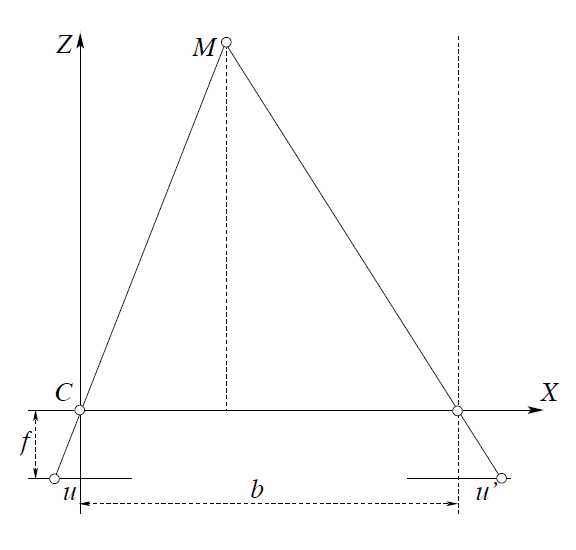
\includegraphics[width=0.6\textwidth]{./figures/Triangolazione_stereoscopica.png}
				\caption{Triangolazione stereoscopica.}
				\label{fig:triangolazione}
			\end{SCfigure}
			
			\noindent e risolvendo si ottiene:

			\begin{equation}
				z=\frac{bf}{u'-u}
				\label{eq:soluzione}
			\end{equation}
			
			\noindent dove $b$ è la distanza tra le due fotocamere, $f$ la focale delle fotocamere e $u'-u$ la distanza fra i due centri ottici.
		
		
		\section{Calcolo delle corrispondenze}
		\label{sec:corrispondenze}
		
			\begin{figure}
				\subfloat[][\emph{Fotocamera di destra.}]
				{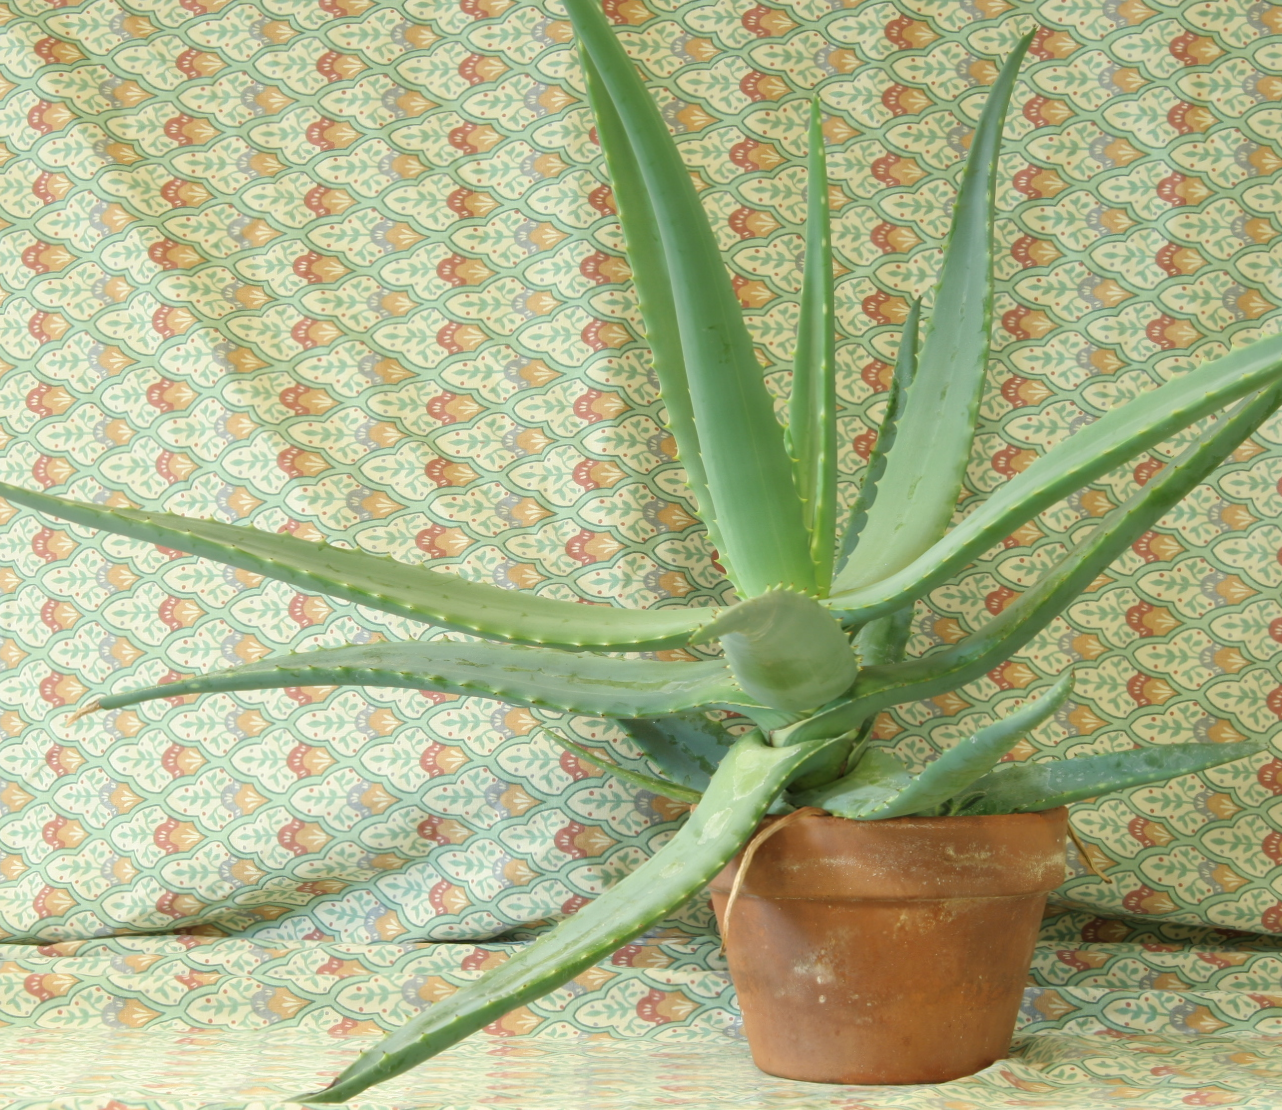
\includegraphics[width=.31\textwidth]{./figures/view1.png}} \quad
				\subfloat[][\emph{Fotocamera di sinistra.}]
				{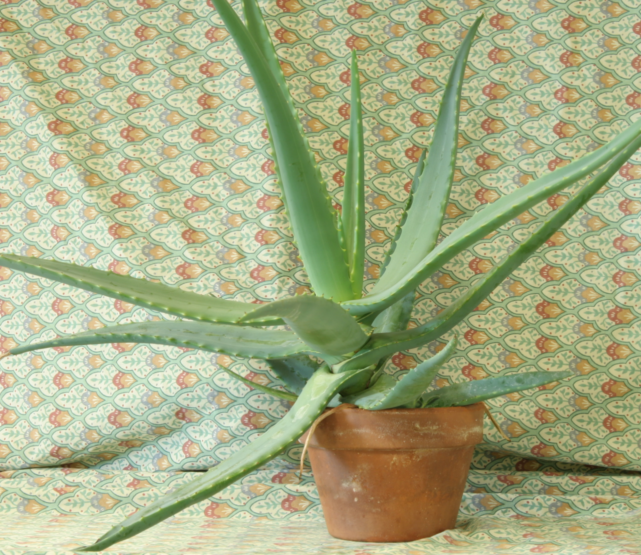
\includegraphics[width=.31\textwidth]{./figures/view5.png}} \quad
				\subfloat[][\emph{Mappa di disparità.}]
				{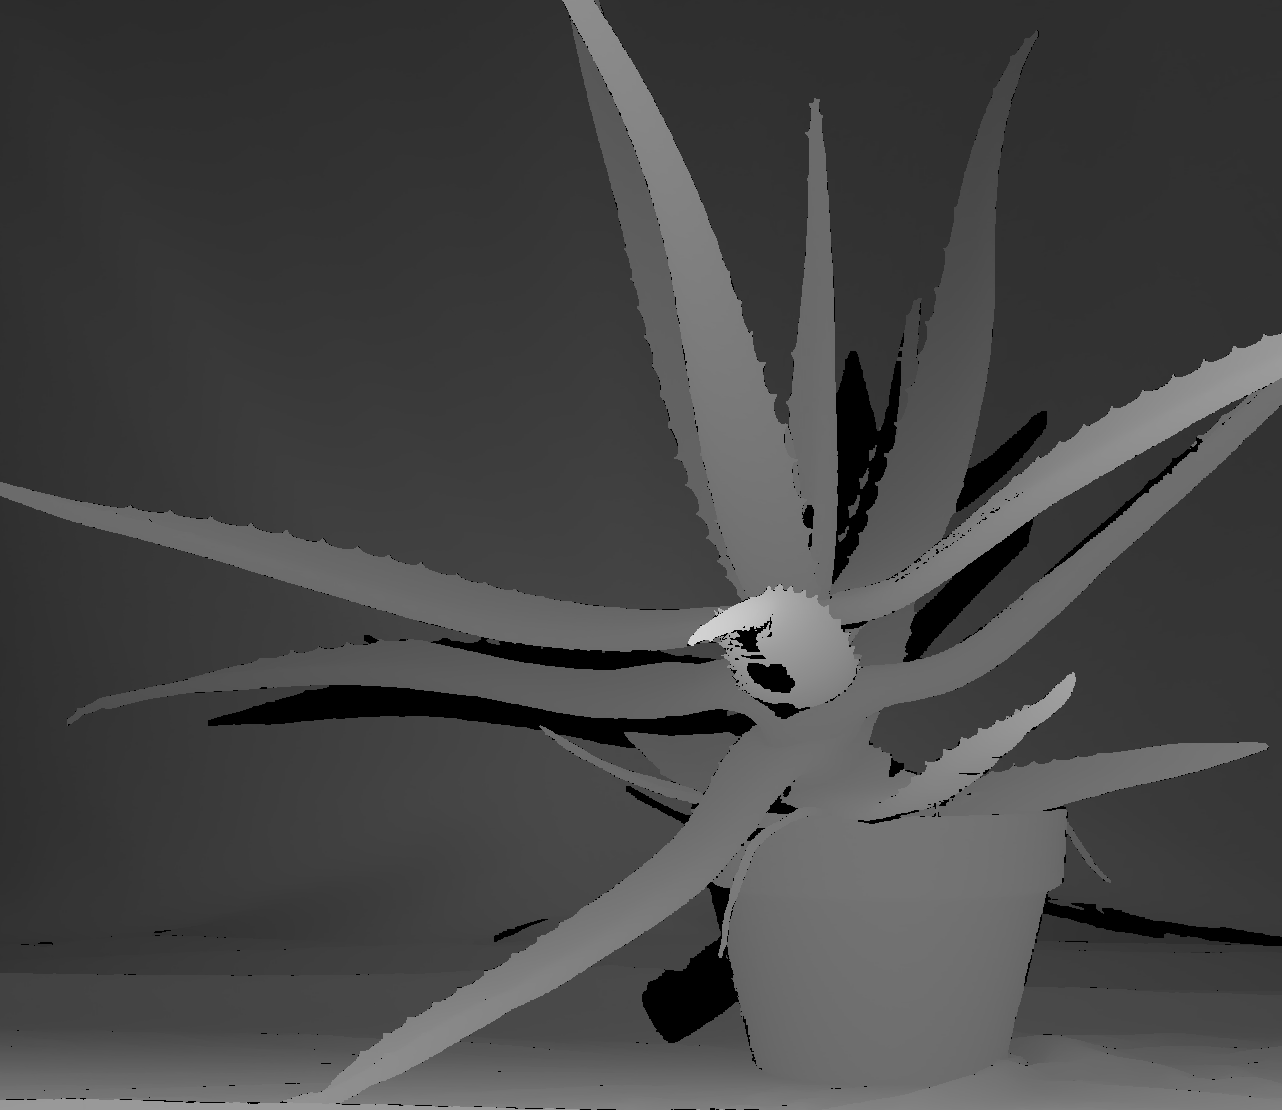
\includegraphics[width=.31\textwidth]{./figures/disp1.png}} 
				\caption{Mappa di disparità con immagine di destra come riferimento, immagine presa da \url{http://vision.middlebury.edu/stereo/data/}.}
				\label{fig:disparità}
			\end{figure}
			
			
			
			Il calcolo delle corrispondenze o della disparità è il problema principale della stereo vision. \newline
			La disparità è la differenza tra due punti coniugati (vettore), immaginando di sovrapporre le due immagini. Il calcolo delle corrispondenze non è altro che il calcolo della disparità per ogni pixel delle due immagini \cite{fusiello}. Si ottiene quindi una mappa di disparità del tipo di figura \ref{fig:disparità}.\newline
			Gli approcci tipici per il calcolo della disparità sono basati su correlazione \cite{correlation} o \textit{semi-global matching (SGM)} \cite{SGM}. In questa tesi viene utilizzato un algoritmo di tipo \textit{SGM}, questo tipo di algoritmi usa una regione dell'immagine al posto del singolo pixel per identificare i punti coniugati. Ogni punto viene confrontato con tutti i punti nella retta epipolare, fino ad ottenere il punto coniugato e quindi la disparità. La disparità però non è una funzione esatta, in quanto la misurazione può essere soggetta da rumore (scarsa o eccessiva illuminazione ecc\dots), oppure l'algoritmo di per se può sbagliare. Viene quindi generata una funzione detta ‘‘funzione di costo’’, la quale ha per ascissa tutti i possibili valori di disparità, e per ordinata la probabilità che quel valore di disparità sia esatto. In realtà, matematicamente parlando, non si ha una probabilità, ed è per questo che si parla di costo. 
			

			



%%--------------------------- MISURE DI CONFIDENZA ------------------------------------%%						
	\nullpage
	
	\chapter{Misure di confidenza}
	\label{sec:confidenza}
	\pagestyle{fancy}
	
		Come accennato nella sezione \ref{sec:corrispondenze}, ad ogni pixel dell'immagine di riferimento (destra o sinistra), viene assegnata una funzione costo, la quale identifica quanto una determinata disparità sia esatta per quel pixel.
			
			
		\begin{figure}[<h>]
			\centering
			\subfloat[][\emph{Funzione costo ideale.}]
			{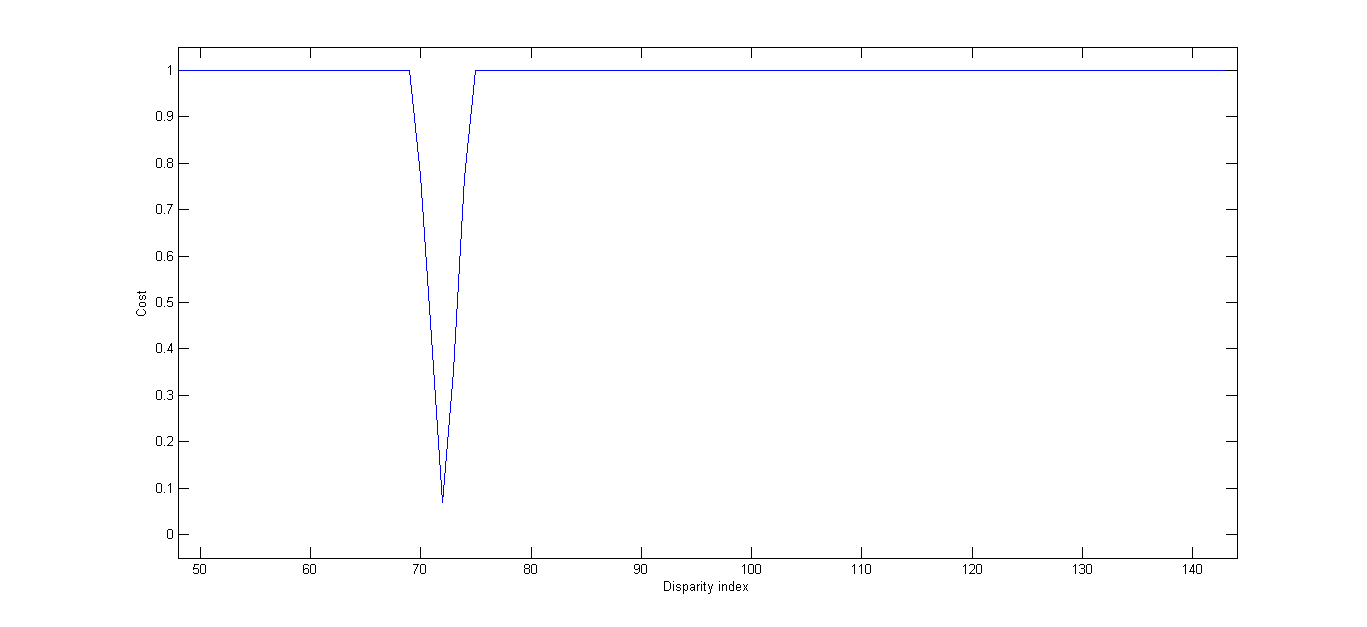
\includegraphics[width=.48\textwidth]{./figures/good_cost.png}} \quad
			\subfloat[][\emph{Funzione costo ambigua.}]
			{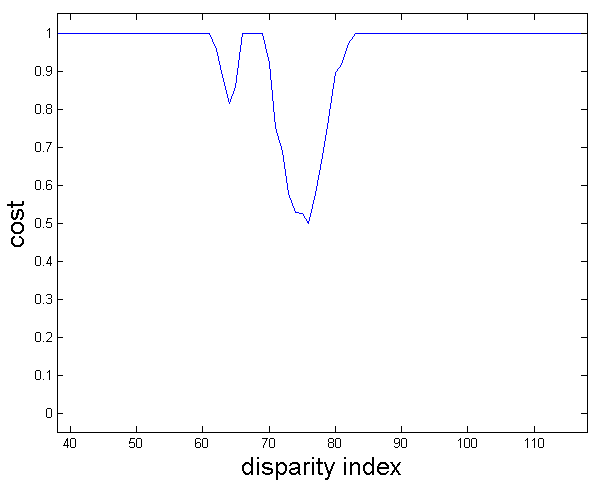
\includegraphics[width=.48\textwidth]{./figures/bad_cost.png}}
			\caption{Due possibili funzioni costo.}
			\label{fig:costi}
		\end{figure}	
		
		\noindent Due possibili funzioni costo sono riportate in figura \ref{fig:costi}. E' chiaro che nel primo caso la disparità  è individuata da quell'unico picco; nel secondo caso invece, la funzione è ambigua, in quanto vi sono diversi picchi, e non è quindi più così banale trovare l'esatta disparità. Si rende quindi necessario lo studio di varie tecniche per misurare la confidenza con la quale viene dato un determinato valore.
		
		
		\section{Implementazione utilizzata}
		\label{sec:implementazione}
		
			Per il calcolo della funzione costo di ciascun pixel, è stato usato un algoritmo di tipo \textit{semi-global matching}, presente nelle librerie open source di visione computazionale \textit{OpenCV} \cite{opencv}. Questo algoritmo, scritto nel linguaggio \textit{C++}, di per se produrrebbe in output solo la mappa di disparità. L'algoritmo è stato quindi opportunamente modificato per poter estrarre la funzione costo di ciascun punto. Si ha quindi in output anche una matrice di formato \textit{.dat}, delle stesse dimensioni dell'immagine originale, ma che ha per ciascuna cella la funzione costo. Successivamente la matrice viene convertita in formato \textit{.mat}, per rendere il tutto più facile da utilizzare con il linguaggio di programmazione \textit{MATLAB}. Poi, con script \textit{MATLAB}, vengono calcolate le confidenze con diverse metriche. Le immagini utilizzate sono state prese dal dataset Midleburry \cite{dataset_2006_1,dataset_2006_2} disponibili su \url{http://vision.middlebury.edu/stereo/data/}. \newline
			Prima di proseguire però, si rende necessario dare alcune definizioni:  		
		
			\begin{itemize}
				\item $c(d)$: il valore del costo assegnato ad una ipotetica mappa di disparità $d$, per un pixel di coordinate $(x,y)$, è denotato con $c(x,y,d)$ o $c(d)$, se le coordinate del pixel non sono ambigue;
			
				\item $c_{1}$: il minimo valore del costo di un pixel è definito con $c_{1}$ e il corrispondente valore di disparità da $d_{1}$; $c_{1}=c(d_{1})=\min\{c(d)\}$;
			
				\item $c_{2}$: con $c_{2}$ viene denotato il secondo valore più piccolo in $d_{2}$, mentre con $c_{2m}$ si denota il secondo minimo locale più piccolo.
				\label{item:definizioni}
			\end{itemize}
			
			Seguono quindi tutte le varie tecniche utilizzate, raggruppate secondo l'aspetto del costo che considerano \cite{indoors_outdoors}.
		
		
		
		\section{Proprietà locali della curva}
		\label{sec:localProperties}	
			In questo genere di metriche, si sfrutta il fatto che la forma della curva di costo intorno al minimo (la nitidezza o la planarità) è indice di certezza nella partita.
			
			\paragraph{Curvature (CUR)}
			\label{par:curvature}
			
				E' largamente utilizzata nella letteratura \cite{indoors_outdoors}, ed è definita come
				
				\begin{equation}
					C_{CUR}=-2c(d_{1})+c(d_{1}-1)+c(d_{1}+1)
					\label{eq:CUR}
				\end{equation} 
			
				\noindent se $d_{1}-1$ o $d_{1}+1$ sono fuori dal range di disparità, il punto minimo $c(d_{1})$ viene usato due volte.
			
			
			\paragraph{Local Curve (LC)} 
			\label{par:local}
			
				Molto simile alla misura \textit{CUR}, la \textit{Local Curve} è descritta da
				
				\begin{equation}
					C_{LC}=\frac {\max\bigr\{ c(d_{1}-1) ,c(d_{1}+1) \bigr\} - c_{1}} {\gamma}
					\label{eq:LC}
				\end{equation}
				
				\noindent il parametro $\gamma$ verrà poi scelto tale da garantire una distribuzione del costo più uniforme possibile tra zero e uno.
			
			
			
		\section{Minimo locale della curva}
		\label{sec:localMinima}	
		
			Si basa sul concetto che la presenza di altri candidati è un'indicazione di incertezza, mentre la loro assenza di certezza.
			
			\paragraph{Peak Ratio Naive (PKRN)} 
			\label{par:PKRN}
		
				A differenza del \textit{Peak Ratio (PKR)}, che calcola il costo con la formula \ref{PKR}
		
				\begin{equation}
					C_{PKR}=\frac{c_{2m}}{c_{1}}
					\label{eq:PKR}
				\end{equation}
			
				\noindent il \textit{PKRN} non richiede che il numeratore sia un minimo locale. Inoltre la formula è leggermente diversa da quella proposta in letteratura \cite{mercedes}
			
				\begin{equation}
					C_{PKRN}=\frac{c_{2} + \epsilon}{c_{1} + \epsilon} - 1
					\label{eq:PKRN}
				\end{equation}
		
				\noindent \textit{PKRN} può essere visto come una combinazione del \textit{PKR} e \textit{CUR}, che assegna bassa confidenza per le corrispondenze con minimi piatti o concorrenti forti. Anche se le modifiche al \textit{PKRN} violano leggermente la metrica originale, ha i seguenti vantaggi rispetto alla controparte originale:
				
				\begin{itemize}
					\item le rare singolarità in cui il denominatore sia nullo non sono più presenti;
					\item piccole variazioni nei costi dovuti al rumore ai livelli bassi del costo, non hanno un forte impatto nella metrica; 
					\item potendo scegliere il valore di $\epsilon$, il range dei possibili valori può essere adattato, al fine di omogeneizzare la misura tra zero e uno.
					\label{item:PKRN}			
				\end{itemize}
				
			
			\paragraph{Nonlinear Margin (NLM)}
			\label{par:NLM}
			
				è definito come
				
				\begin{equation}
					C_{NLM}= e^{ \frac{ c_{2}-c_{1}} {2\sigma_{NLM}^2}}-1
					\label{eq:NLM}
				\end{equation}
				
				\noindent le variazioni del parametro $\sigma_{NLM}$ verranno poi discusse nel capitolo \ref{sec:risultati}.
				
		\section{Intera curva}
		\label{sec:entireCost}
		
			Questi metodi convertono la funzione costo in una distribuzione di probabilità sulla disparità.
			
			\paragraph{Maximum Likelihood Metric (MLM)}
			\label{par:MLM}
			
				Insieme a \textit{PKRN} è una delle metriche più promettenti. Entrambe hanno ottenuto risultati sopra la media sia su immagini indoor che outdoor \cite{indoors_outdoors}.
				La \textit{Maximum Likelihood Metric} è definita come
				
				\begin{equation}
					C_{MLM}= \frac{e^\frac{-c_{1}}{2\sigma_{MLM}^2}}{\sum_{d} e^\frac{c_{i}}{2\sigma_{MLM}^2}}
					\label{eq:MLM}
				\end{equation}  	
			
				\noindent In questo caso $\sigma_{MLM}$ rappresenta l'incertezza della disparità, e anche per questo caso la sua variazione verrà discussa nel capitolo \ref{sec:risultati}.
		
				
		\section{Consistenza fra disparità di destra e sinistra}
		\label{sec:leftRight}
			
			Questa tipologia di misure consiste nel fatto che, idealmente, un punto nella mappa di disparità destra dovrebbe essere lo stesso nella mappa di disparità sinistra. Fin ora abbiamo denotato la disparità con $c(x,y,d)$, ma per chiarezza chiameremo $c_{R}(x_{R},y,d_{R})$ la disparità ottenuta tenendo come riferimento l'immagine di destra. Questo genere di misure risulterà più complicata delle precedenti, in quanto prima di calcolare la disparità "finale", si rende necessario calcolarla prima sia per l'immagine di destra che quella di sinistra. Per il calcolo delle due mappe di disparità, in questa tesi è stato usato l'algoritmo \textit{Sum of Absolute Differences (SAD)}. Questo algoritmo è di tipo \textit{block matching}, cioè calcola la mappa di disparità confrontando non il singolo pixel ma blocchi di pixel. Nel nostro caso le finestre hanno dimensione di $(2n+1)\times(2m+1)$
		
			\begin{equation}
				c_{SAD}(x,y,d)=\argmin_{d}\biggr\{\sum_{(k,l)}\abs[\big]{I_{R}(x+k,y+l) - I_{L}(x+k+d,y+l)}\biggr\}
				\label{eq:SAD}
			\end{equation}		
			
			\noindent dove $k\in[-n,n]$, $l\in[-m,m]$ e $I(x,y)$ indica il livello di grigio del pixel $(x,y)$ dell'immagine destra ($I_{R}(x,y)$) o sinistra ($I_{L}(x,y)$). 
		
		
			\paragraph{Left Right Consistency (LRC)}
			\label{par:LRC}
			
				E' l'unico metodo che viene utilizzato in questa tesi per quanto riguarda la consistenza fra disparità di destra e sinistra.
				\textit{Left Right Consistency (LRC)} viene calcolato prendendo il valore disparità calcolato in una immagine, e proiettandolo nell'altra immagine. Se la differenza nei valori è inferiore a una determinata soglia, allora il pixel è occluso. Questo procedimento viene poi ripetuto anche al contrario, cioè proiettando la seconda immagine nella prima. Inoltre il costo di \textit{LRC} viene calcolato come segue:
				
				\begin{equation}
					C_{LRC}(x,y)=\abs[\big]{d_{1}-D_{R}(x-d_{1},y)}
					\label{eq:LRC}
				\end{equation}	
				
				\noindent con $d_{1}=\argmin_{d}\bigr\{c(x,y,d)\bigr\}$ e $D_{R}(x-d_{1},y)=\argmin_{d_{R}}\bigr\{c_{R}(x-d_{1},y,d_{R})\bigr\}$.
				
				
%%--------------------------- RISULTATI ----------------------------------------------%%

	\chapter{Risultati}
	\label{sec:risultati}
	\pagestyle{fancy}				
	
		Tutte le misure effettuate vengono confrontate con una mappa di disparità chiamata \textit{ground truth}. Questa mappa è sempre disponibile nei dataset utilizzati \cite{dataset_2006_1, dataset_2006_2}, per tutte le immagini e per tutte le risoluzioni. La disparità \textit{ground truth} viene calcolata utilizzando sempre una coppia di videocamere, ma aggiungendo anche uno o più proiettori che illuminano la scena con dei pattern specifici. Ogni telecamera utilizza quindi i pattern per determinare un codice univoco per ciascun pixel. Trovare quindi le corrispondenze si traduce banalmente nel verificare quali pixel delle due immagini hanno lo stesso codice \cite{ground_truth}.  			
		
		\begin{SCfigure}[\sidecaptionrelwidth][h!]
			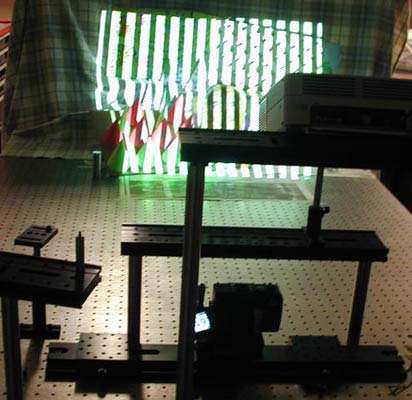
\includegraphics[width=0.5\textwidth]{./figures/ground_truth.png}
			\caption{Configurazione del proiettore e della coppia di videocamere per il calcolo della disparità ground truth; si può notare come il proiettore illumina la scena con dei pattern diversi per facilitare il compito delle videocamere.}
			\label{fig:groundtruth}
		\end{SCfigure}
		
		\noindent Prima di continuare definiamo l'errore di disparità come
		
		\begin{equation}
			e_{d}=\abs{d_{GT}-d}
			\label{eq:errore}
		\end{equation} 
		
		\noindent Dove $d_{GT}$ è la disparità \textit{ground truth} e $d$ sono i valori di disparità ottenuti. \newline Per valutare la capacità delle misure di confidenza di predire dove una disparità è corretta, è stato creato uno script \textit{MATLAB} che ordina prima tutte le disparità ottenute in ordine decrescente di confidenza, e poi ne calcola l'errore con densità crescente. Quindi, per ogni misura di confidenza ordinata secondo il valore di disparità, viene selezionato il primo 5\% e si calcola l'errore medio in due modi:  
		
		\begin{enumerate}
			\item Nel primo metodo si misura la percentuale di pixel che ha un errore di disparità maggiore di uno;
			
			\item Nel secondo si misura semplicemente l'errore medio per ogni pixel.
			\label{enum:errore}
		\end{enumerate}
				
		\noindent Si ripete poi con il 10\% e così via sino al 100\%. Prima di confrontare le varie metriche si è pero' trovato il parametro ottimale per quelle con parametri variabili.
		
		\section{Variazione parametri}
		\label{sec:parametri}
		
			In questa sezione, prima di confrontare le misure, verificheremo quali parametri sono più adatti per quelle che dipendono da tali. Consideriamo quindi la \textit{Local Curve}, \textit{Peak Ratio Naive}, \textit{Nonlinear Margin}  e \textit{Maximum Likelihood metric}.
		
			\paragraph{Variazione parametro $\bm{\gamma}$ per \textit{LC}}
			\label{par:gamma}
		
				Ora indagheremo quali effetti produce la 
		
		
				\begin{wrapfloat}{figure}{l}{0pt}
					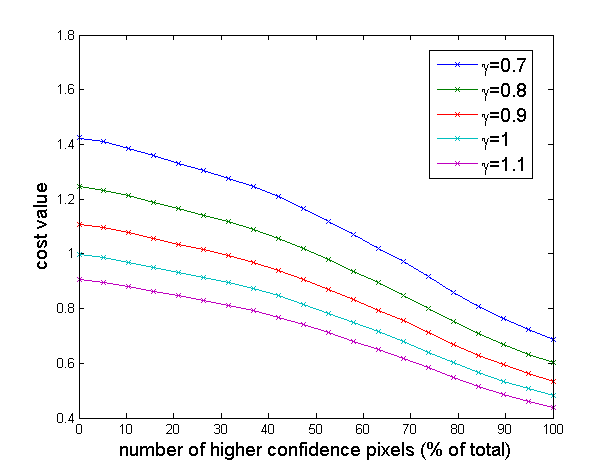
\includegraphics[width=0.5\textwidth]{./figures/gamma_LC.png}
					\caption{Distribuzioni diverse con valori di $\gamma$ diversi.}
					\label{fig:gammaLC}
				\end{wrapfloat} 
		
				\noindent variazione  del parametro $\gamma$. Come prima cosa si è osservato per quale valore si ha una distribuzione più uniforme tra $0$ e $1$. Come si può vedere dalla figura \ref{fig:gammaLC}, si ha una migliore distribuzione per $\gamma=0.9$. Per quanto riguarda l'errore medio invece, si ottengono risultati lievemente migliori per valori di $\gamma$ più elevati. Questi però influiscono molto sulla uniformità della misura; ad esempio con $\gamma=2$ si migliora solo di un inezia l'errore medio, ma la distribuzione apparterrà poi a un intervallo compreso tra circa $0,24$ e $0,5$. Come valore finale si è quindi deciso per un $\gamma$ pari a $0,9$. \newline
		
			\paragraph{Variazione parametro $\bm{\epsilon}$ per \textit{PKRN}}
			\label{par:epsilon}
		
				Come prima, verifichiamo come si comporta la distribuzione della funzione al cambiare del parametro $\epsilon$. Si nota che per valori minori di $1$ di $\epsilon$ il costo massimo supera $1$, mentre con valori troppo grandi si ha poca variazione tra il costo massimo e minimo. Il caso migliore si ha per un $\epsilon$ compreso tra $1,1$ e $1,2$, per semplicità scegliamo il valore $1,1$. 
			
				\begin{wrapfloat}{figure}{l}{0pt}
					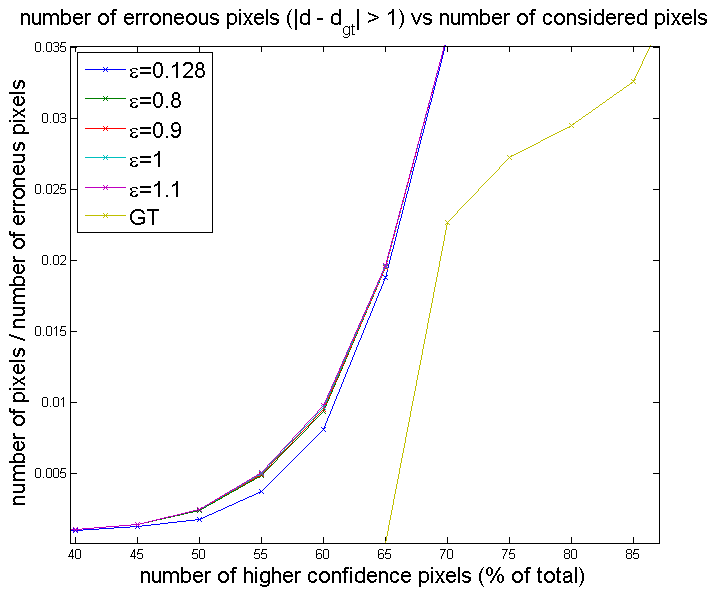
\includegraphics[width=0.5\textwidth]{./figures/epsilon_PKRN.png}
					\caption{Distribuzioni diverse con valori di $\epsilon$ diversi.}
					\label{fig:epsilonPKRN}
				\end{wrapfloat} 
			
			
				\noindent Per quanto riguardagli errori rispetto la \textit{ground truth}, i valori per il quale $e_{d}$ è maggiore di uno non  subiscono praticamente nessun cambiamento al variare di epsilon. Si hanno invece piccole variazioni per quanto riguarda l'errore medio, migliorando per $\epsilon$ grandi, ma non tali da giustificare un tale peggioramento della distribuzione fra $0$ e $1$. Il valore finale resta $1,1$. \newline \newline \newline \newline
	
			\paragraph{Variazione parametro $\bm{\sigma}$ per \textit{NLM}}
			\label{par:sigmaNLM}
			
				Ripetiamo ancora una volta il procedimento, i risultati sono pressoché simili a prima, cioè grosse variazioni di distribuzione e trascurabili variazioni di errore per differenti valori di $\sigma$. Dopo qualche tentativo con diversi parametri, si arriva alla conclusione che i risultati migliori si ottengono con $\sigma_{NLM}=0,9$.
				
			\paragraph{Variazione parametro $\bm{\sigma}$ per \textit{MLM}}	 	 	
		 	 \label{par:sigmaMLM}
		 	 
		 	 	Questa ultima misura è molto più sensibile alle variazioni parametriche, i risultati migliori in questo caso si sono ottenuti con $\sigma_{MLM}=0,25$.
		 	 	
		\section{Confronto delle misure}
		\label{sec:confronto}		 	 	  
		
			\begin{figure}[!h]
				\subfloat[][\emph{Disparità calcolata con algoritmo \textit{SGM}.}]
				{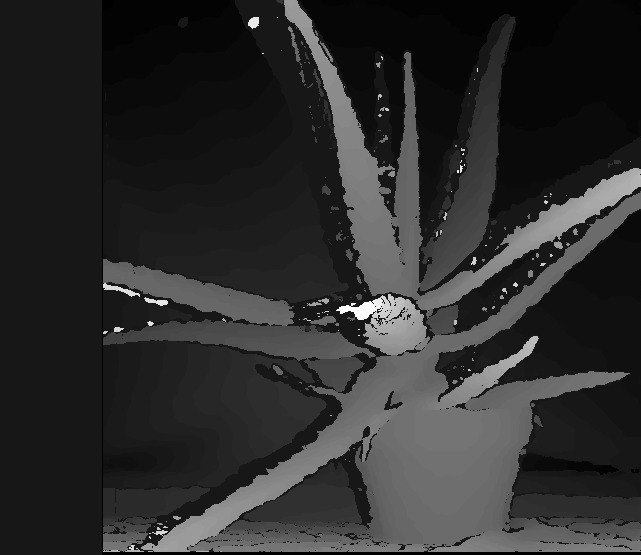
\includegraphics[width=.31\textwidth]{./figures/D_SGM.png}} \quad
				\subfloat[][\emph{Misura Curvature.}]
				{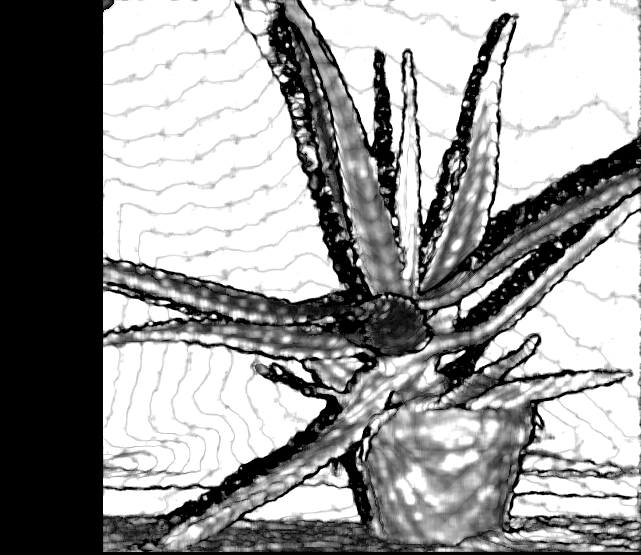
\includegraphics[width=.31\textwidth]{./figures/CUR.png}} \quad
				\subfloat[][\emph{Misura Local Curve.}]
				{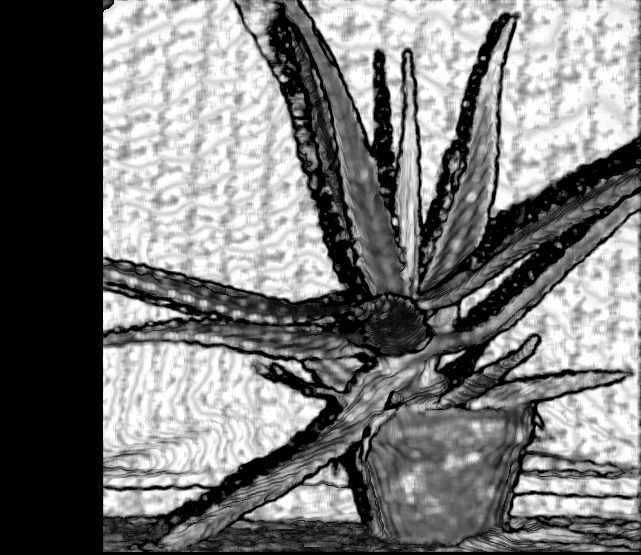
\includegraphics[width=.31\textwidth]{./figures/LC.png}} \quad 
				\subfloat[][\emph{Misura Peak Ratio Naive.}]
				{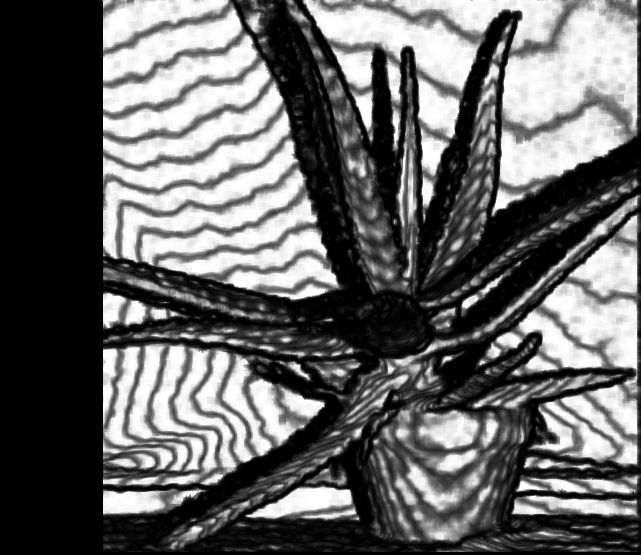
\includegraphics[width=.31\textwidth]{./figures/PKRN.png}} \quad
				\subfloat[][\emph{Misura Nonlinear Margin.}]
				{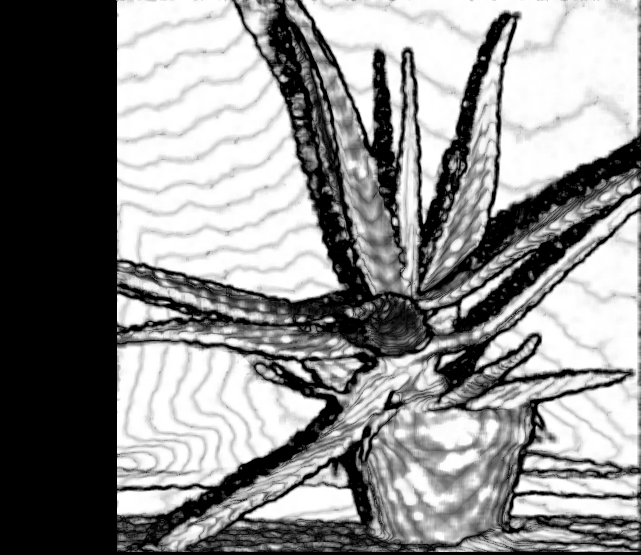
\includegraphics[width=.31\textwidth]{./figures/NLM.png}} \quad
				\subfloat[][\emph{Misura Maximum Likelihood metric.}]
				{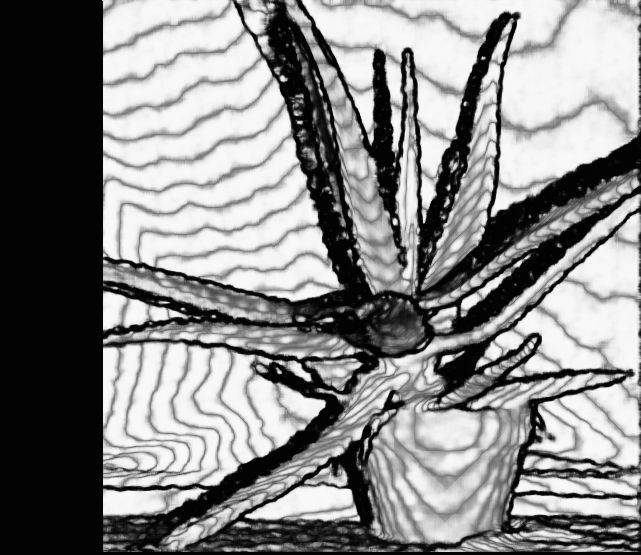
\includegraphics[width=.31\textwidth]{./figures/MLM.png}}
				
				\caption{Disparità e relative misure di confidenza.}
				\label{fig:disparità&costi}
			\end{figure}
			
			Cominciamo dal dire cosa aspettarci dai due confronti descritti prima. Per il primo grafico ci aspettiamo di trovare una curva che resta a zero per una determinata percentuale di confidenze, e che  poi tende a crescere in maniera pressoché lineare per le successive.  
			


%%--------------------------- COMBINAZIONE DI MISURE ------------------------------------%%						
	
	\chapter{Combinazione di misure}
	\label{sec:combinazione}
	\pagestyle{fancy}
				
		Per combinazione di misure, si intende il combinarne più insieme al fine di migliorarne i risultati. Considerando le misure di confidenza come probabilità, la cosa più semplice da fare sarebbe quella di dire che, essendo indipendenti, la loro combinazione non è altro che il loro prodotto. In realtà però, non è del tutto corretto definirle indipendenti, in quanto tutte dipendono dalla stessa ‘‘matrice dei costi’’, calcolata con il medesimo algoritmo (in questo caso \textit{SGBM}). 
		
	
	
	
%%---------------------------- APPENDICI ----------------------------------------%%	
	\nullpage	
	\appendix 
	\addcontentsline{toc}{chapter}{Appendici}
	
	\chapter{Codice MATLAB utilizzato}
	\label{sec:codice}
	
		In questa appendice viene riportato solo il codice \textit{MATLAB} che calcola le mappe di disparità con le varie tecniche descritte nel paragrafo \ref{sec:confidenza}; si riporta inoltre il codice utilizzato per analizzare i risultati ottenuti.
	
		\section{computeConfidence.m}
		\label{sec:computeConfidence}
		
			Questo script computa la mappa di disparità per \textit{MSM}, \textit{CUR}, \textit{LC}, \textit{PKRN}, \textit{NLM} e \textit{MLM}.
	
			\lstinputlisting[basicstyle=\scriptsize]{./code/computeConfidence.m}
		
		\newpage
		\section{leftRightConsistency.m}
		\label{sec:leftRightConsistency}
			\lstinputlisting[basicstyle=\scriptsize]{./code/leftRightConsistency.m}	
			
		\newpage
		\section{funcSADL2R.m}
		\label{sec:funcSADL2R}
			\lstinputlisting[basicstyle=\scriptsize]{./code/funcSADL2R.m}
			
		\newpage
		\section{funcSADR2L.m}
		\label{sec:funcSADR2L}
			\lstinputlisting[basicstyle=\scriptsize]{./code/funcSADR2L.m}		




%%---------------------------- BIBLIOGRAFIA ----------------------------------------%%
	\nullpage
	
	\begin{thebibliography}{1}
	\label{bibliografia}
	\addcontentsline{toc}{chapter}{Bibliografia}
		
		\bibitem{fusiello}
		A. Fusiello,
		\emph{Visione Computazionale, appunti delle lezioni},
		\url{http://profs.sci.univr.it/~fusiello},
		2008.

		\bibitem{mercedes}
		D. Pfeiffer, S. Gehrig, N. Schneider,
		\emph{Exploiting the Power of Stereo Confidences},
		IEEE Conference on Computer Vision and Pattern Recognition, 2013.
	
		\bibitem{correlation}
		D. Scharstein, R. Szeliski, 
		\emph{A taxonomy and evaluation of
		dense two-frame stereo correspondence algorithms}, 
		IJCV,47(1-3):7–42, 2002.
		
		\bibitem{SGM}
		H. Hirschmüller, 
		\emph{Accurate and efficient stereo processing
		by semi-global matching and mutual information}, 
		IEEE CVPR, pages 807–814, San Diego, USA, June 2005.
		
		\bibitem{mordohai_pami}
		X. Hu, P. Mordohai,
		\emph{A Quantitative Evaluation of Confidence Measures for Stereo Vision},
		IEEE Transactions on Pattern Analysis and Machine Intelligence, 2012.
		
		\bibitem{indoors_outdoors}
		X. Hu, P. Mordohai,
		\emph{Evaluation of Stereo Confidence Indoors and Outdoors},
		IEEE Conference on Computer Vision and Pattern Recognition (CVPR), San Francisco, USA, June 2010.
		
		\bibitem{dataset_2006_1}
		D. Scharstein, C. Pal,
		\emph{Learning conditional random fields for stereo},
		IEEE Computer Society Conference on Computer Vision and Pattern Recognition (CVPR 2007), Minneapolis, MN, June 2007.
		
		\bibitem{dataset_2006_2}
		H. Hirschmüller, D. Scharstein,
		\emph{Evaluation of cost functions for stereo matching},
		IEEE Computer Society Conference on Computer Vision and Pattern Recognition (CVPR 2007), Minneapolis, MN, June 2007.
		
		\bibitem{opencv}
		\emph{OpenCV library 2.4.9},
		\url{http://opencv.org/}.
		
		\bibitem{ground_truth}
		D. Scharstein, R. Szeliski,
		\emph{High-Accuracy Stereo Depth Maps Using Structured Light},
		Proc. CVPR, volume I, pages 195–202, 2003.
		
		


		
	\end{thebibliography}


\end{document}